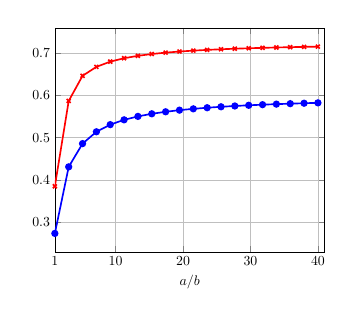
\begin{tikzpicture}[scale=0.5]
\begin{axis}[xlabel=$a/b$,ymajorgrids=true,xmajorgrids=true,xmin=1,xmax=41,xtick={1,10,20,30,40}]
%%%%%%%%%%% NATURAL CONFIGURATION
\addplot[Blue,mark=*,very thick] coordinates {(1.0,0.272727272727) (3.05263157895,0.430693069307) (5.10526315789,0.485809682805) (7.15789473684,0.513853904282) (9.21052631579,0.530839231547) (11.2631578947,0.54222972973) (13.3157894737,0.550398839739) (15.3684210526,0.556543837357) (17.4210526316,0.561334087055) (19.4736842105,0.56517311609) (21.5263157895,0.568318666049) (23.5789473684,0.570943075616) (25.6315789474,0.57316594743) (27.6842105263,0.575072886297) (29.7368421053,0.576726777816) (31.7894736842,0.578174856414) (33.8421052632,0.579453289276) (35.8947368421,0.580590238365) (37.9473684211,0.581607959129) (40.0,0.582524271845) };
%%%%%%%%%%% MODIFIED CONFIGURATION
\addplot[Red,mark=x,very thick] coordinates {(1.0,0.384615384615) (3.05263157895,0.587044534413) (5.10526315789,0.646666666667) (7.15789473684,0.667894413751) (9.21052631579,0.680272108844) (11.2631578947,0.688379573784) (13.3157894737,0.694101508916) (15.3684210526,0.698355754858) (17.4210526316,0.70164281929) (19.4736842105,0.704258862717) (21.5263157895,0.706390328152) (23.5789473684,0.7081604426) (25.6315789474,0.709653916211) (27.6842105263,0.71093090049) (29.7368421053,0.712035286704) (31.7894736842,0.712999852442) (33.8421052632,0.713849569803) (35.8947368421,0.714603798297) (37.9473684211,0.715277777778) (40.0,0.715883668904) };
\end{axis}
\end{tikzpicture}
%%% Local Variables:
%%% mode: latex
%%% TeX-master: "../../mainManuscript"
%%% End:
